\documentclass{article}
\usepackage[utf8]{inputenc}
\usepackage{indentfirst}
\usepackage[export]{adjustbox}
\usepackage{setspace}
\usepackage[margin=1.2in]{geometry}
\graphicspath{{images/}}
\usepackage{afterpage}
\newcommand*{\TitleFont}{%
      \usefont{\encodingdefault}{\rmdefault}{b}{n}%
      \fontsize{70}{70}%
      \selectfont}

\title{ 
\includegraphics[width=15cm]{uc3m-logo.jpg} \\ \TitleFont USER INTERFACES \\ Case Study: Campus Global\vspace{7cm}}
\author{Héctor Otero Mediero NIA: 100316516 \\  Daniel Medina García NIA: 100316850 \\ Diego Vicente Martín NIA: 100317150 \\ Alejandro Rodríguez Salamanca NIA: 100315874}
\begin{document}
\begin{titlepage}
\end{titlepage}
\maketitle
\thispagestyle{empty}
\newpage
\doublespace
\tableofcontents
\thispagestyle{empty}
\newpage
\singlespace
\section{Main	objective	of	the	system	to	design}

In this case study we will analyze, redesign and implement is \textbf{Campus Global} . The reason we chose it over the other option, the {\it Renfe} website, is that we use Campus Global on a normal basis and its design stands out, in a bad sense, as different from the pages that belong to the same entity and that link to it. In addition to this, it will make our analysis different due to its uniqueness. 


Campus Global is the website, only accessible to university students and teachers, that allows you to check your official score reports, exam dates and all the processes you have opened with the university. It also shows you information about current events that might interest you. The problem that will be analyzed throughout this report is that this great idea of having all your official information in one site has a poor execution which is highlighted by the good design of other university pages that link to it. Furthermore, the site doesn't offer any facility in terms of navigating through it which we'll be able to see in the analysis of the process of looking up your average mark in Campus Global.

\section{End	users	of	the	system}

Campus Global is accessed by the students and majority of the personnel of the university. This implies the end user is with a high likelihood an individual with a relatively high level of computer and navigation expertise. Nonetheless, the tasks a end user performs in this website don't entail any complex activity. In most cases, the user will use Campus Global only to read official information, therefore it should be pretty straight-forward how to do so. As we will see, this is not true and the user will need clairvoyance in order to find the information needed.

\section{Website Analysis}
\subsection{Login page}

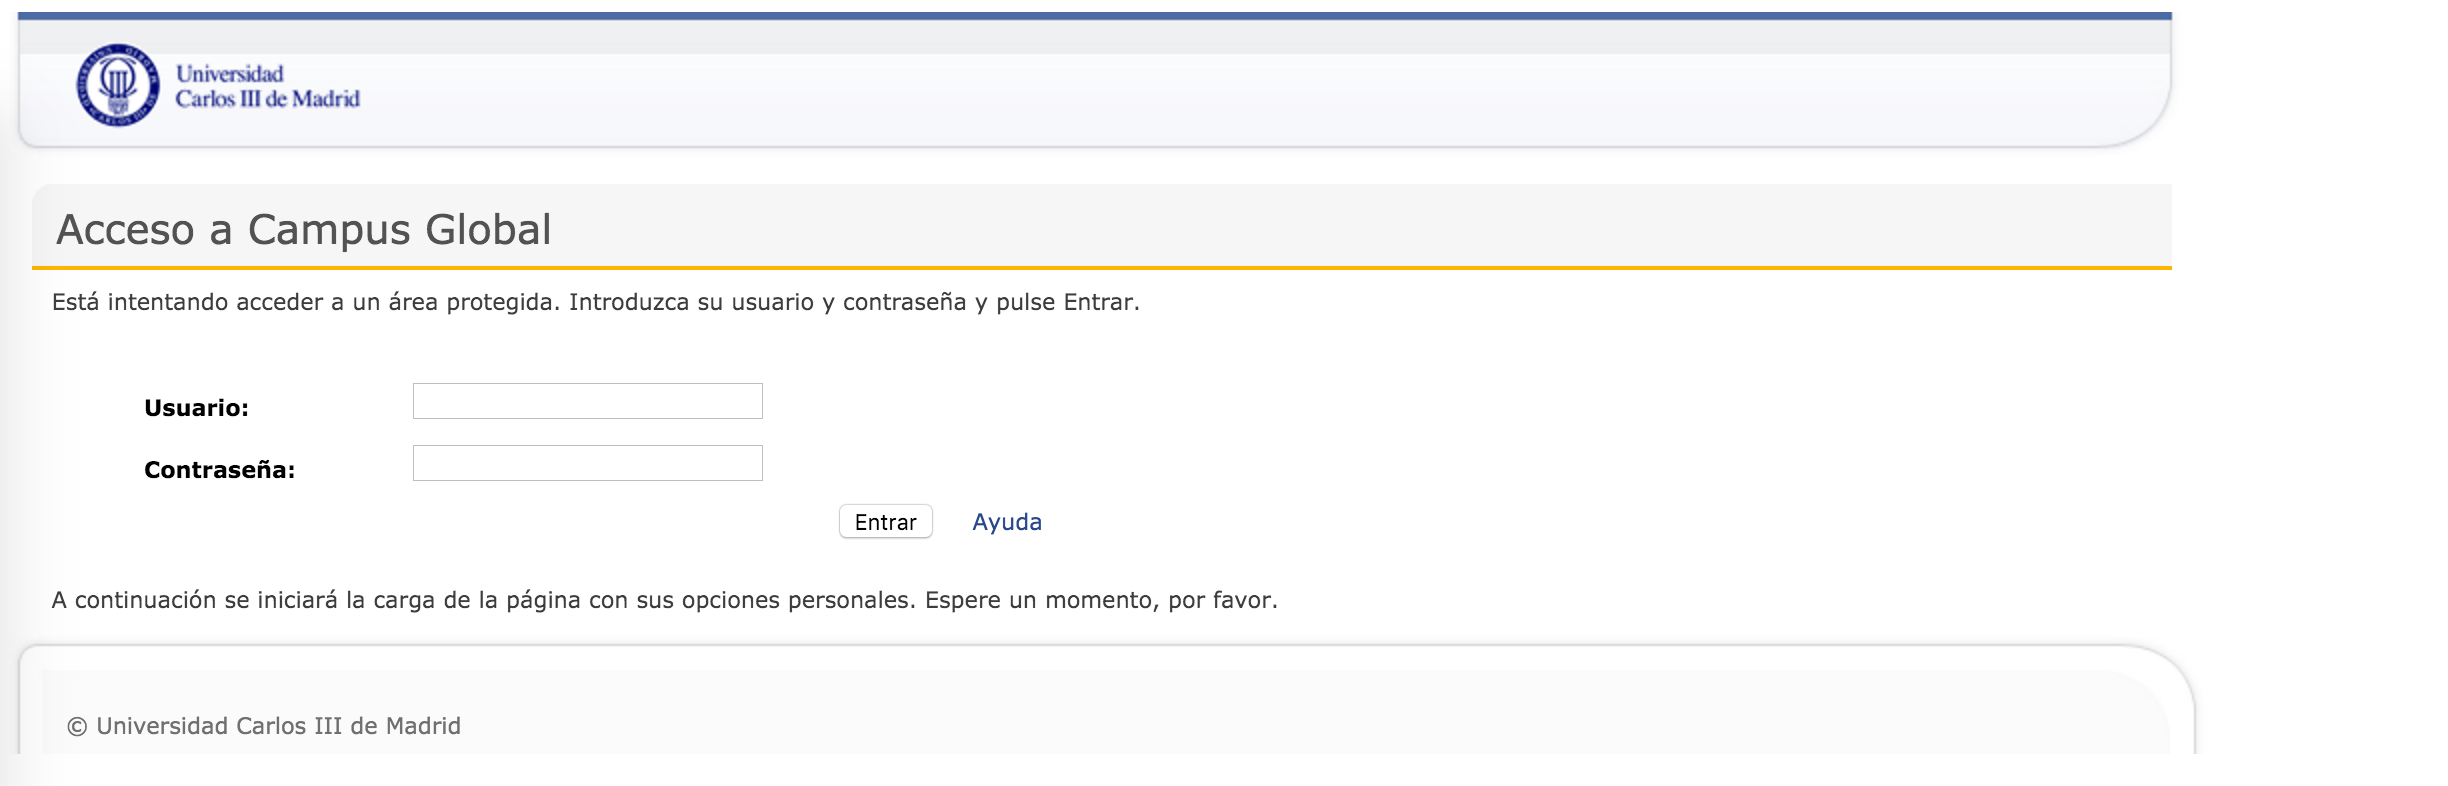
\includegraphics[width=15cm, height=10cm, keepaspectratio]{loginpage} 


The first fact that strikes the user is that even if you’re coming from a English-configured webpage or have your browser preferences set to English, the login page will \textbf{only be displayed in Spanish}. No option appears in the page either with regard to changing this setting, nor the Ayuda link will help you with understanding this page. Thus, the text displayed above and below the fields won’t be understandable for every not-spanish-speaking user that sees the page. This behavior will continue for every page in Campus Global.


Leaving behind the language, we find a page whose \textbf{content display and aesthetic are poor}.
Firstly, we find a low resolution university logo. In most displays nowadays, this logo will be contemplated as pixelated which seems to be a prolepsis of how the content will be displayed inside the site. 
Below this logo, we find the fields for the username and password. Its left-alignment added up to the selection of colors used in the page, gives it a feeling of emptiness. Furthermore we find the login button (with a default design) to the right of this fields, rather than below which would be the expected. This completes the overall sensation that this page wasn't designed and implemented with a lot of care.

\subsection{Homepage}
\vspace{0.3cm}
\begin{center}
\includegraphics[width=15cm, height=10cm, keepaspectratio]{campus}
\end{center}


Once we login, we see the following homepage. We find again an easily analyzable poor design. 

The \textbf{header and footer} of the page get \textbf{all the user attention} since they have a flashy orange background that doesn’t fit with any of the other pages or style of the current page.  
The central content isn’t aligned with the header or footer which signals a careless implementation of the page. 

The organization of the components in the row below the header is strange for the nowadays user as, usually, the login information is on the upper right corner, rather than on the left one. The position of the search bar is the correct one, but once again there’s \textbf{no alignment} with the button of search (whose appearance could be improved also).  On the left of the search bar, we found the links to other pages (Biblioteca, Directorio, Incidencias, Opina and Ayuda) which are located in a strange position, as one may think they are categories on these page rather than links to other pages. 

On the left side of the pages, we find a menu with what seems to be categories and subcategories inside the page. The names chosen for each section are in the most part ambiguous and we can find repeated information or links that lead to unnecessary navigation, which points out the \textbf{little efficiency of use} of the website. But what makes the menu worse is the inconsistency, as more than half of the sections will drive you out of Campus Global. The other ones are the real categories and subcategories. Some of them are simply \textbf{empty pages} as we can see in the example below, with \textbf{not a single useful error message} about what the problem is at all.

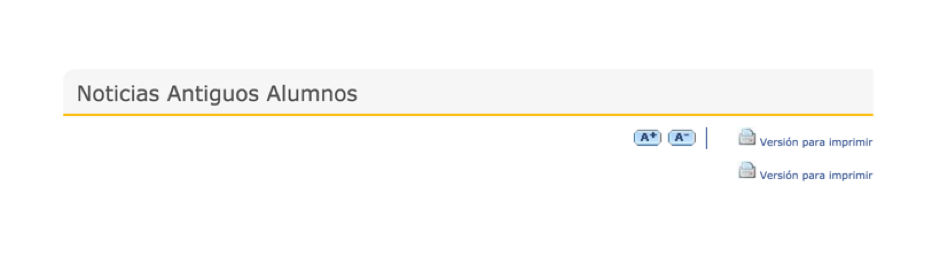
\includegraphics[width=15cm, height=10cm, keepaspectratio]{noticiasantiguos}
As a last element of the menu we find \textbf{“Mis aplicaciones frecuentes”} this is a good choice of design as it offers shortcuts to frequent users, but the placement is not the best and the algorithm running behind doesn’t work most of the time.


To the right of the menu we find two columns, one under the name of “Avisos”. Its design consists of a list of events. Below each event we find a undescriptive text and a date. This date, rather than being the date when the event will take place, is the date when the event was updated which leads to confusion.

On the far right side 5 distinct areas. We will simply pose the following questions about each one.
\textbf{Emergencias}, what’s the difference between this and the top right link \textit{Incidencias}? \textbf{Comunicación institucional}, isn’t this information on the link of the bottom? (\textit{Información y contacto}).
\textbf{Importante para Estudiantes}, so \textit{Avisos} aren’t important?
\textbf{Te Interesa}, what’s the difference between \textit{Importante para Estudiantes}, \textit{Avisos} and this, and what’s supposed to interest me.
\textbf{Agenda}, are there only two events in the upcoming days?\\

While navigating the website, we will sometimes (like when we click the “Servicios” category) find a “Edit” button on the upper left corner that will allow us to change the view from “Graphical” to “List”. As we can see below the results are horrific and we doubt this is supposed to be enabled. 
\vspace{0.5cm} \\
\includegraphics[width=15cm, height=10cm, keepaspectratio]{edit} 
\vspace{0.5cm} \\
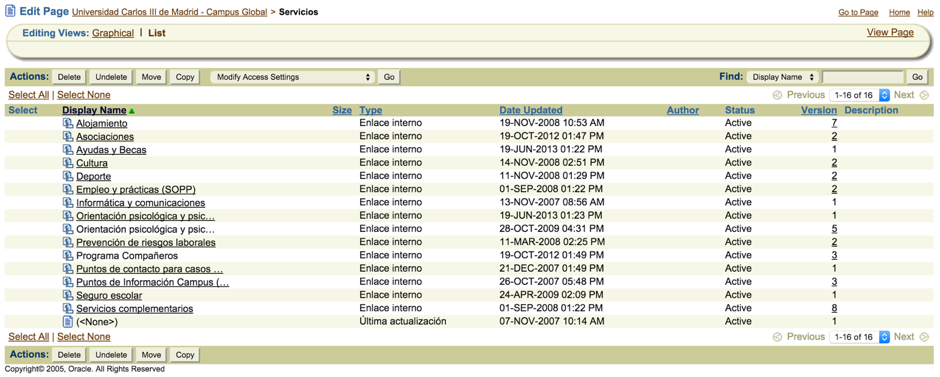
\includegraphics[width=15cm, height=10cm, keepaspectratio]{editresult}


\subsection{Student’s average mark query}
There are two ways we could approach this query:
One would be scattering through the categories section. First we would go to “Estudiantes”, then to “Información Personal” followed by “Expediente, notas provisionales, nota media” which would lead out of Campus Global (Is there any information stored in this place?!), then we would click on “Consulta de la nota media” which would take us to the next page where the \textbf{most important link of the page}, and the one we’re looking for, is placed where you would least expect it, \textbf{hidden in the right margin}. That makes it a total of 5 pages visited (and 3 different domains) in order to obtain one of the most important things Campus Global offers. No efficiency at all.

\includegraphics[width=15cm, height=10cm, keepaspectratio]{personalinformation} \vspace{0.3cm} \\
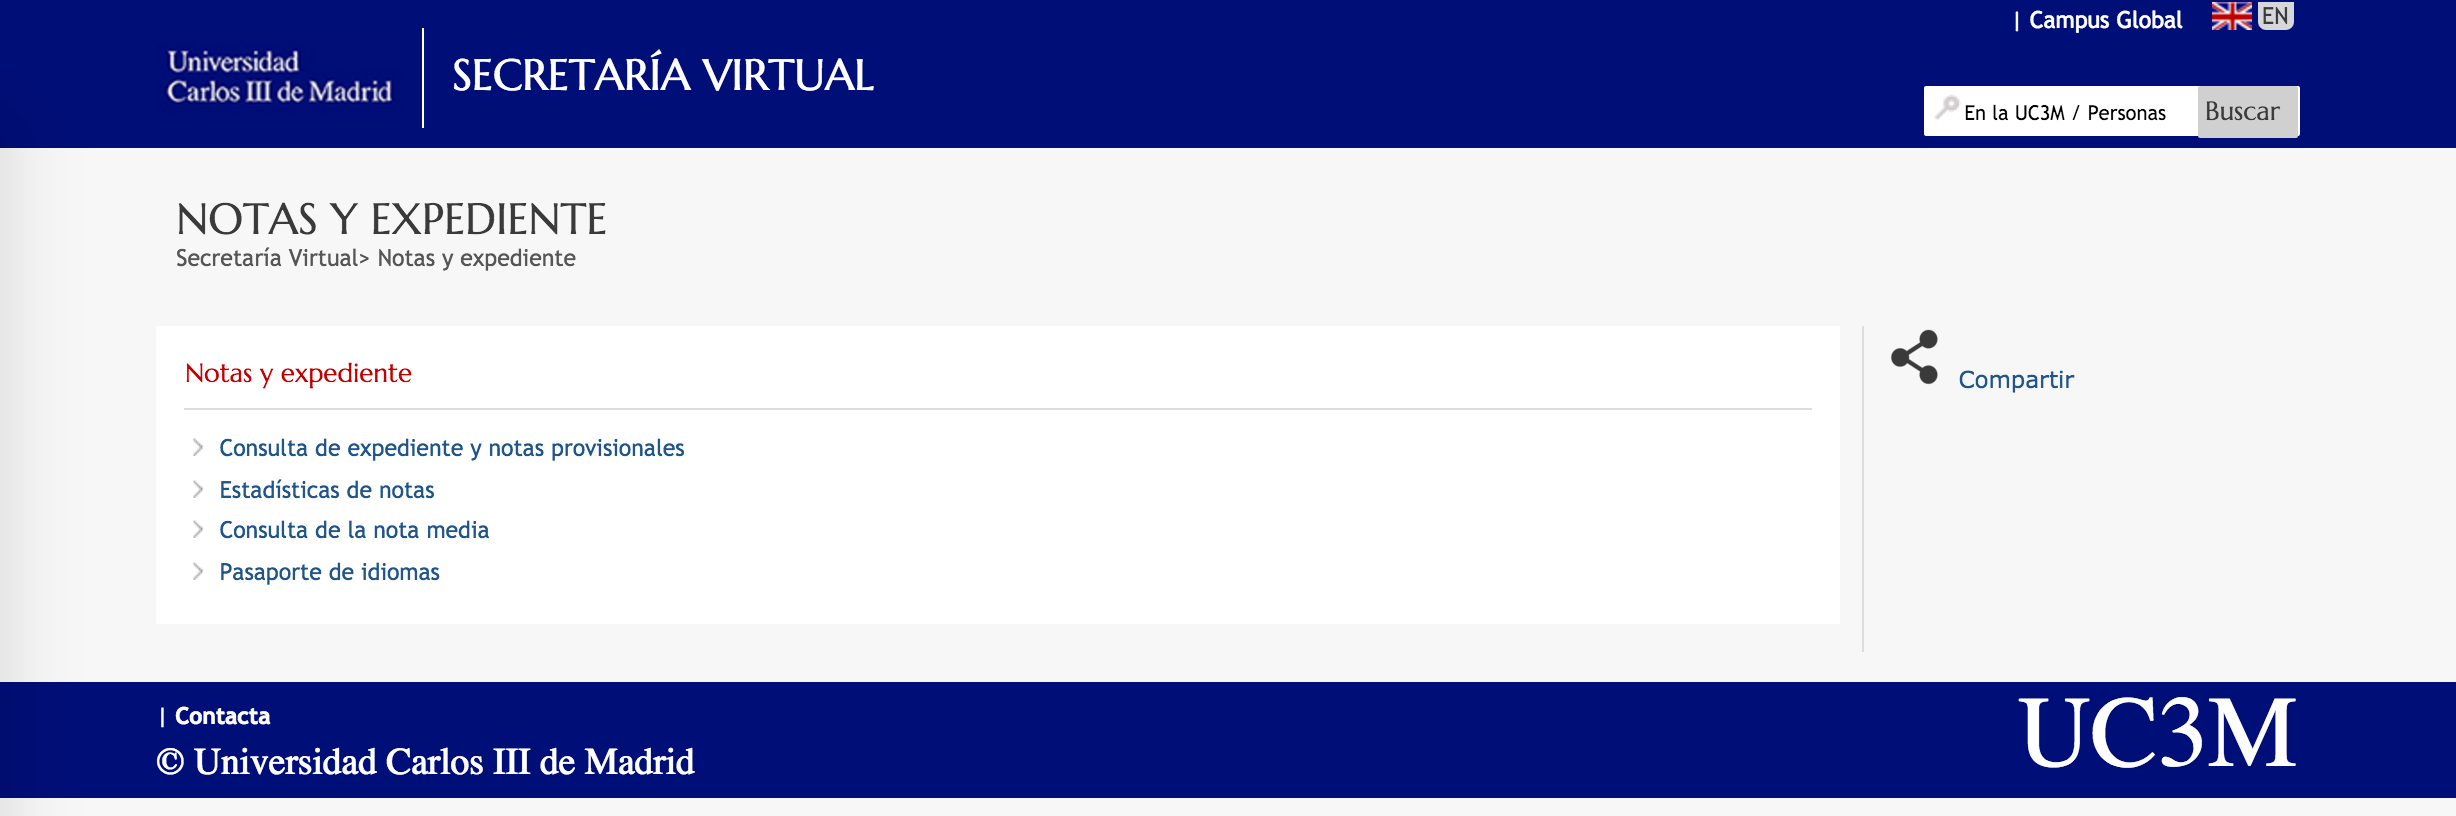
\includegraphics[width=15cm, height=10cm, keepaspectratio]{notasyexpediente} \vspace{0.3cm} \\
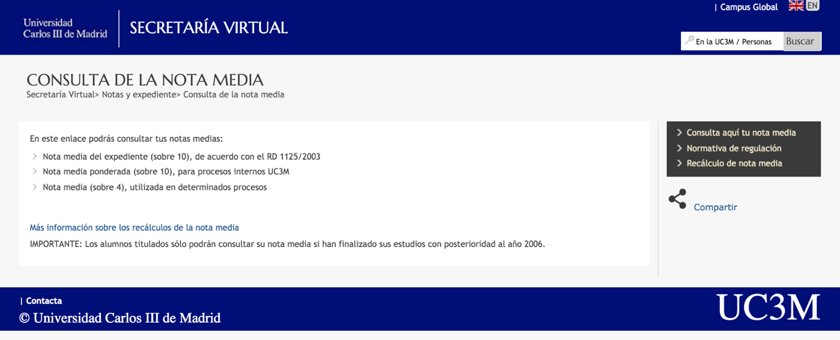
\includegraphics[width=15cm, height=10cm, keepaspectratio]{consulta}\vspace{0.3cm} \\



The first way would be used if you manage to follow correctly all the links, which, unless you are used to it, is near impossible. So, you would have another option: looking up “Average mark” on the search bar (you actually need to look up “Nota media” as the site is in Spanish). So, let’s analyse the pages you go through in order to get there.
\subsection{Search result page}

When we search “Nota media” the results found are divided in two sections: 
The results themselves, where we see a first link saying “Consulta de la nota media”, which is self-descriptive (and that will be the chosen) and two others with the same title that lead to different places and which by the title the user wouldn’t have any idea of what’s behind those links. 
Related content. This idea is great, as if you were looking for example for the criteria of a certain subject or your exams date or schedule, you could be prompted with the official PDF with the information right below your search. Unfortunately, this is not what happens. The related content to the user’s average mark seems to be some files related to the Telecommunications major from 2001 and 2004. 
\begin{center}
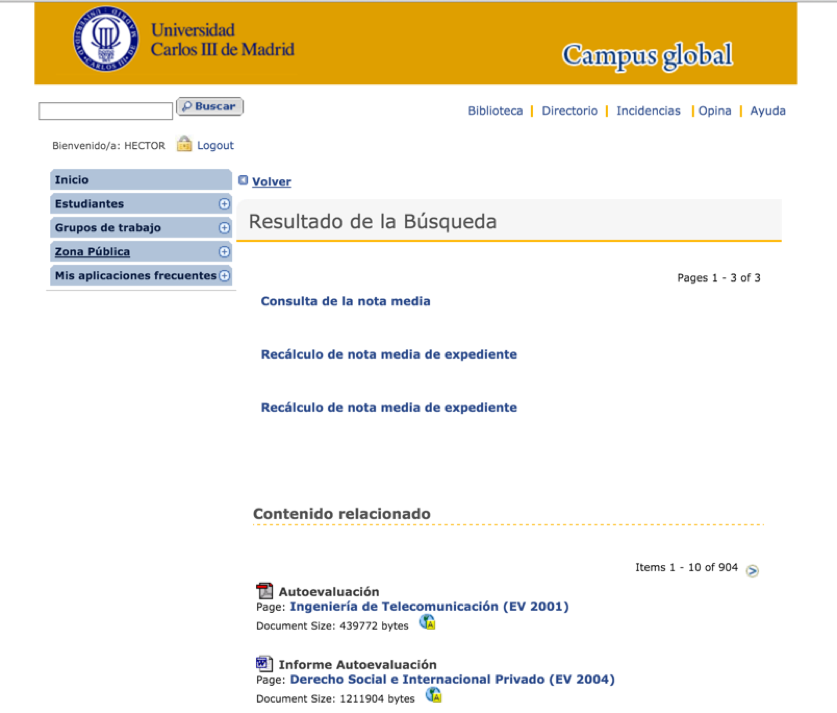
\includegraphics[width=15cm, height=10cm, keepaspectratio]{busqueda}\vspace{0.3cm} \\
\end{center}

When we click “Consulta de la nota media”, we’re taken to another page (different from any page visited during the first process) where we have to click a link on the right margin to get to the Grades page. Again this shows a very bad choice of placement of important information for the user.
\begin{center}
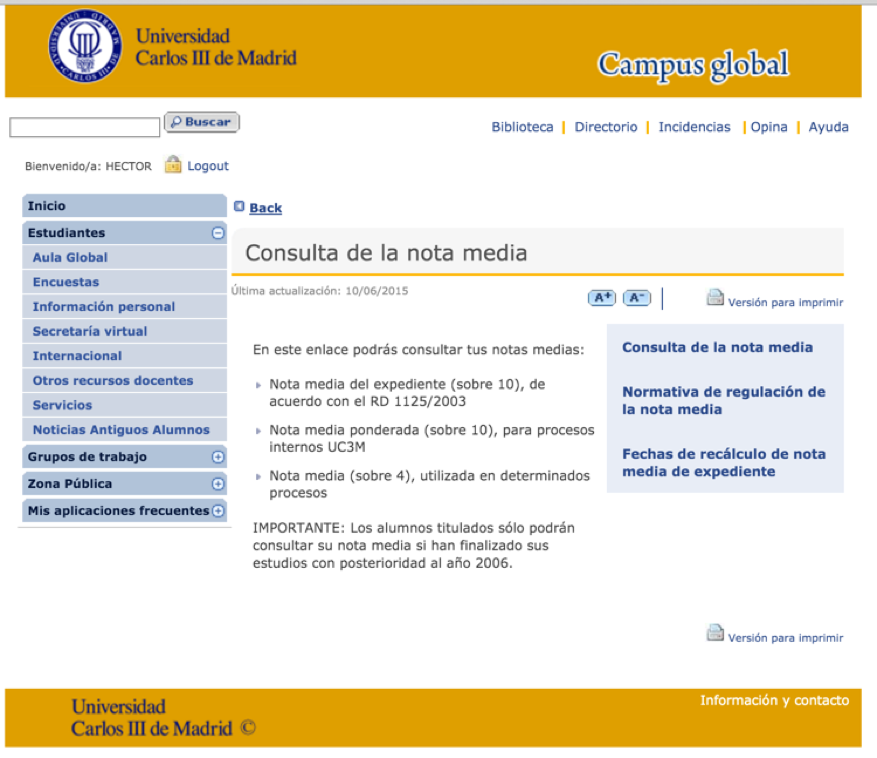
\includegraphics[width=10cm, height=10cm, keepaspectratio]{2}\vspace{0.3cm} \\
\end{center}













\subsection{Average mark page}
Once we finally arrive to the Average Mark page, we see a page that doesn’t have the most aesthetic and minimalist design, but which shows the information we’re looking for with detail, explaining what each mark means. This page repeats some of the errors we’ve pointed out in previous pages (alignment of the content, style consistency…) and adds a new one. We find in the top right corner a “Power button” which we may think makes you logout of the page and takes you back to Campus Global or to uc3m.es. Well that is not correct, it simply removes the information related to the average mark. Clicking this button again will make the information appear again. \vspace{0.2cm} \\
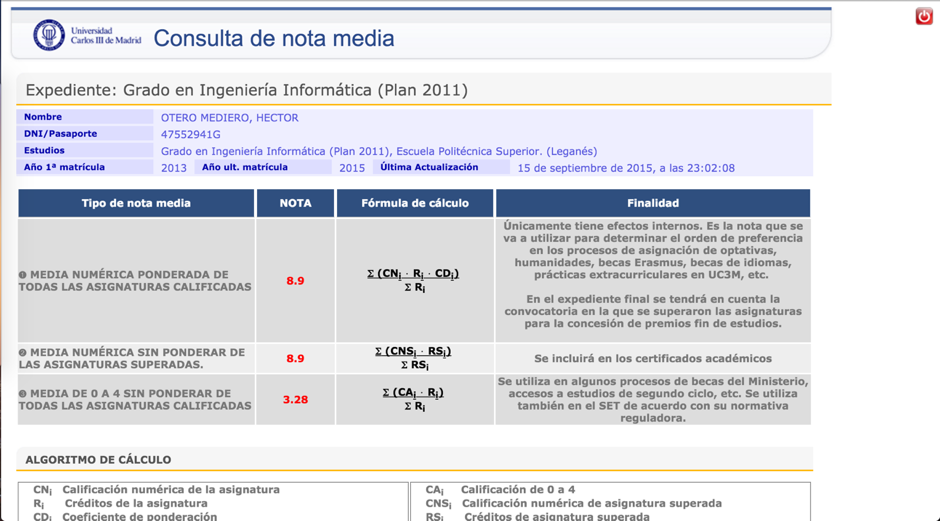
\includegraphics[width=15cm, height=10cm, keepaspectratio]{notamedia}\vspace{0.3cm} \\
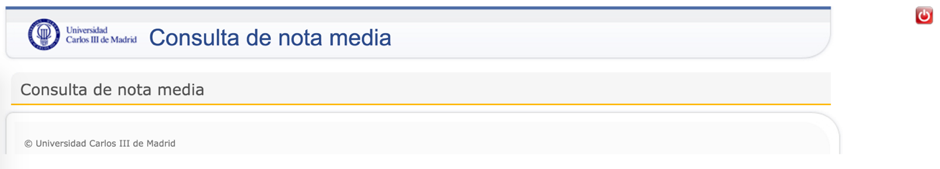
\includegraphics[width=15cm, height=10cm, keepaspectratio]{power}\vspace{0.3cm} \\





\newpage



\section{Justification of our design}
\subsection{Introduction}
Following the integration within the overall aesthetics of the university’s site, we’ve come up with a new design that addresses the aforementioned problems backing up our decisions with the so-called web design patterns defined by Van Duyne. The different patterns will be referenced by the capital letter and number assigned in Van Duyne’s guide.
We’ll proceed now to explain our design decisions when designing the new page in the same order we’ve analysed in the previous section.

As an overall analysis of the new design, we can see how the content has been adjusted to a grid \textbf{(I1)} solving the problems of the alignment in the previous design. We’ve adjusted the content depending on the width of the screen as it previously gave an impression of emptiness most of the time \textbf{(I4)}. Content-wise the page has been designed consistently, this is, all the pages in the site follow a similar design having the header, footer and menus in every one of them. We’ve also tried to adapt the content organization so the attention is directed where we intend to \textbf{(I3)} and to display meaningful error messages rather than the usual “Page not found” displayed in the previous design \textbf{(K13)}.
\subsection{Log in page}

To start with, we have placed both input boxes in the centre of the page, with bigger, clearer labels, in a much more intuitive and fast-to-find architecture. We’ve also introduced the two tonalities of blue from uc3m.es so the user keeps feeling the site belongs to the university space. In the functional part of the design, the login operation will be identified as a secure sign in in the site \textbf{(E3)}. We’ve also included a question mark on the top right of the sign-in box that will indicate the user what’s needed in order to login to the site.
Less accessed information is displayed in the bottom of the page, which includes the university name and a new “Language selection” option selection which we found necessary to add as, otherwise, foreign students may face difficulties when accessing their data \textbf{(D10)}. We’ve put special focus in highlighting this information without breaking the minimalist style of the whole page, by changing the background colour of this footer to the same as the input division. In addition to the language selection, there are two links on the footer of the page that will be constant across the whole site. They are, the privacy policy of the site as well as a “About us” of the university itself. \textbf{(E4, E5)}
\subsection{Homepage}
The header contains the same image as uc3m.es site in the same colours and quality (giving the site style continuity to uc3m.es) \textbf{(D1)}, adding the Global Campus label to follow, as we want to make clear what the site offers \textbf{(C2)} . The UC3M logo will appear in several parts of each page apart from the header in every page of the site \textbf{(E1)}. The user name as well as the Logout button are in a clearly identified division, on the right side of the window, where users are used to have their account-related information nowadays. 

Secondly, a new horizontal menu, placed below the header image. \textbf{(K2)} The categories appearing will be different from those in the original left-side menu, as they were confusing and used ambiguous terms to define different categories. They’ll be organized hierarchically (from more general topics, to concrete ones). Main ones, in separated boxes, followed by an extra box including the previous small horizontal menu with 5 options and some more links which were wandering around in the former design \textbf{(B2, B3)}. In this category we will include all those leading to sites different from Campus Global \textbf{(K7, K8, K10)}, so that similar actions lead to similar consequences for the user. Each of the boxes will show a list of the options in such section under it on hover (or on click), making visible for the user the list of subcategories available inside that category \textbf{(H6)}. 
Beneath the menu but still near the top of the page we can find the Search Bar \textbf{(B1)}, occupying the whole width of the section for higher visibility, whose results page will be addressed later on. It provides a predictive input with the previous searches made by the \textbf{(H11)}.

Here is where we get to the main section, similar to a message board. This one shares content with the old one, whilst having little in common regarding the presentation. A card-based design will show the articles from the preceding right sections “Important for students” and “May interest you” \textbf{(B7)}  in the first positions, followed by the ones from the foregoing middle section below. Each card will have a similar structure, a photo related to the topic, a clear headline explaining the topic and a description \textbf{(D3)}.

Besides this principal card area, we’ve added a secondary section in the right. This one will display an intuitive calendar showing clearly the events from the former “Agenda” section. Underneath the calendar, we can find the new place where “May interest you” links are placed. It will include frequently visited places by the user inside the site, offering a personalized view that will reduced the navigation time \textbf{(H1)} for the habitual users.

Finally we find the footer. Instead of an image repeating the information of the header, we will use this space to provide the user with contact links, legal information and emergency links, properly organised so the user doesn’t get overwhelmed. As in the first times you visit the website, some common questions may arise among the users, we’ve gathered them in a FAQs section, accessible from the last category on the right \textbf{(H7)}. Just as closure, following the uc3m.es design we also include the uc3m name in the right of the footer.

We’ve got rid of the edit option as, in an intention of offering the user the possibility of making the content display differently \textbf{(H9)}, that customization didn’t achieve any improvement in the website.


\subsection{Search result page}
Our goal in the design of the search is to minimize the number of steps needed to retrieve the information the user is looking for. Giving the possibility of jumping from subcategories to direct results or simply looking up from the homepage \textbf{(J1)}. The search results will be made much more accurate (J3) and possible in several languages. Since we thought it was idea having a direct link to the files that the user could be looking for, we’ve included this inside the results. Not all results have a file linked to them, but the ones who do have the most general one. For example, if you look up for Non-European Mobility, the pdf linked would be the basis.
Remembering the processes done in the website analysis. Since the categories have been redesigned, we wouldn’t have that long and tiring navigation, and in a couple of clicks we would have the information required displayed. The search results are shown in the mockup made. They are quality and concrete results.
\subsection{Grades page}
We’ve performed little design changes to this page, since the content was the one needed and the display was correctly organized. We’ve simply updated the look for a more modern one, adapting it to the one of the rest of the pages.

\end{document}
